\subsubsection{\LIME ir \gls{mca} metodų sintezės tikslumo nustatymas}

Šio eksperimento tikslas yra nustatyti autoriaus siūlomos modifikuoto \LIME ir \gls{mca} metodų sintezės \glsplko{adversarial} aptikimui tikslumą. Kaip ir praeitame eksperimente, \ref{fig:exp3:confusion}-ame pav. pateikiamos dvi klasifikavimo lentelės -- išskiriant ir neišskiriant \textit{obfuskuotą} klasę. 

\begin{figure}[h]
    \begin{subfigure}{0.5\textwidth}
        \centering
        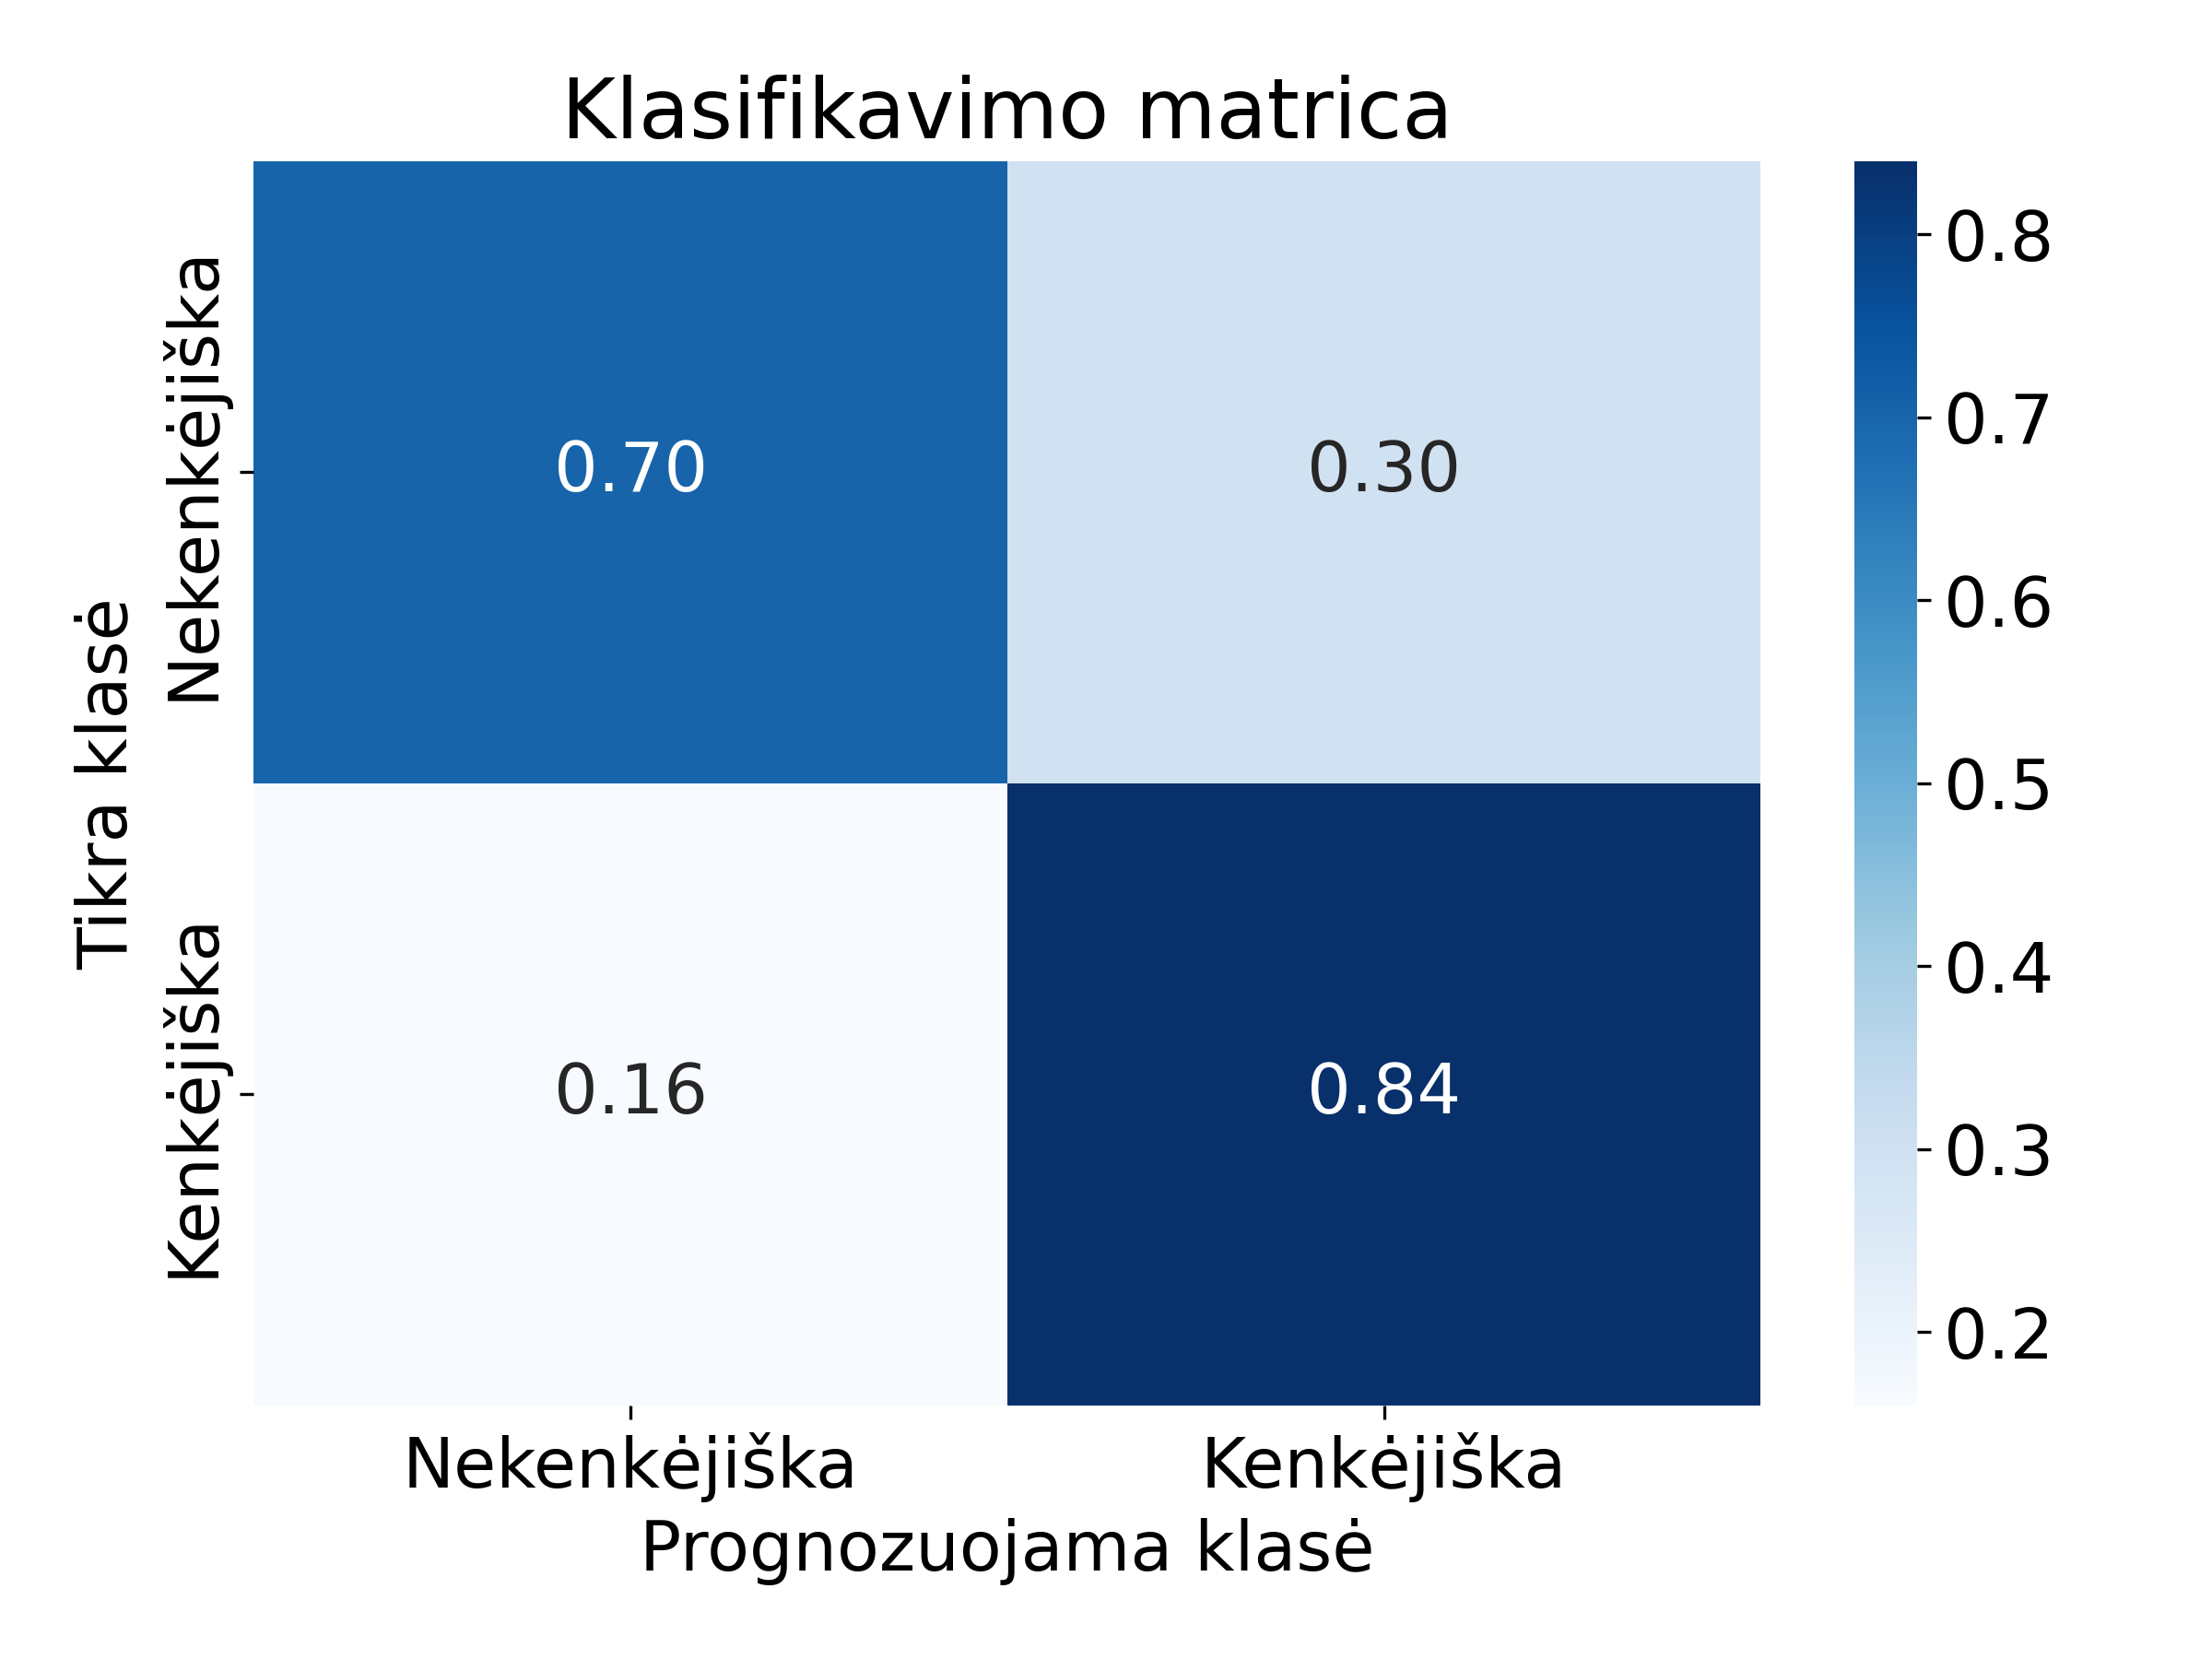
\includegraphics[width=\textwidth]{images/synthesis_2x2.png}
        \caption{Neišskiriant \textit{obfuskuotų} pavyzdžių klasės}
    \end{subfigure}
    \begin{subfigure}{0.5\textwidth}
        \centering
        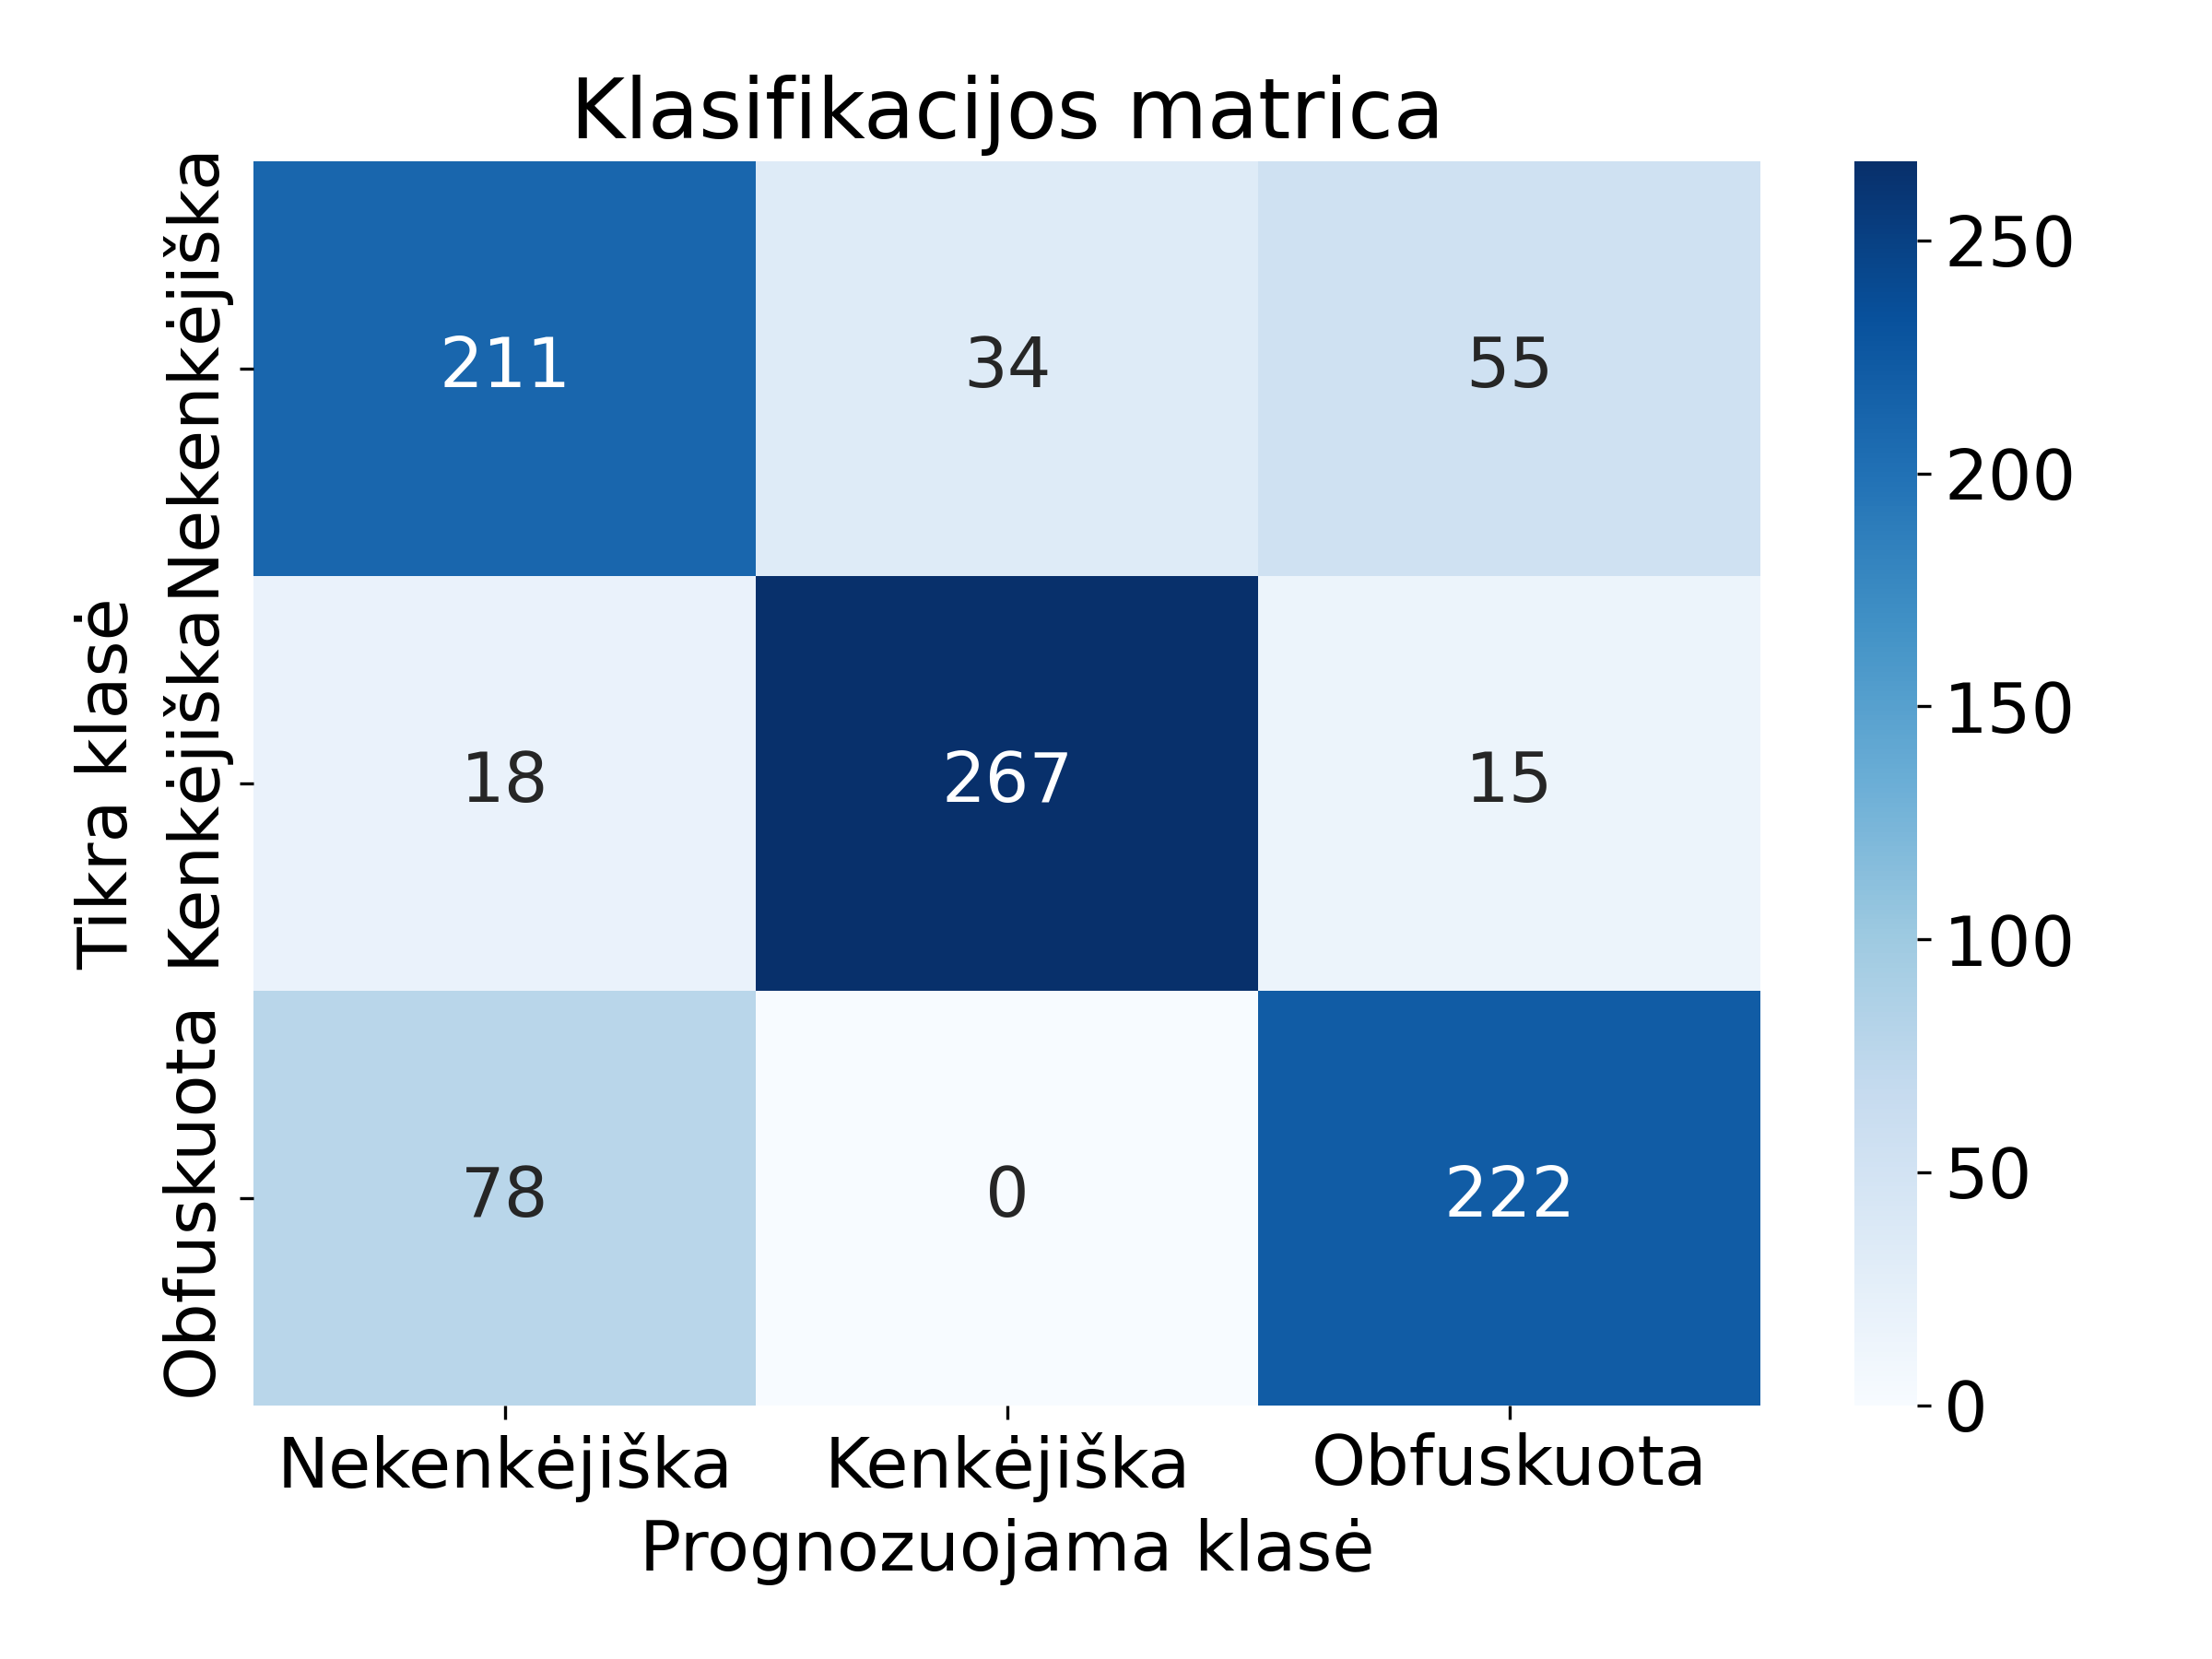
\includegraphics[width=\textwidth]{images/synthesis_3x3.png}
        \caption{Išskiriant \textit{obfuskuotų} pavyzdžių klasę}        
    \end{subfigure}
    \caption{\LIME ir \gls{mca} metodų sintezės klasifikavimo lentelės}
    \label{fig:exp3:confusion}
\end{figure}

\begin{table}[h]
    \caption{TODO}
    \centering
    \exptable[\accLime]{tables/synthesis_2x2.csv}
    \label{tbl:exp3:metrics2}
\end{table}

\begin{table}[h]
    \caption{TODO}
    \centering
    \exptable[\accLimeObf]{tables/synthesis_3x3.csv}
    \label{tbl:exp3:metrics3}
\end{table}

% Show results with original method